En la revisión de literatura, podemos encontrar el simulador 
"Lunar Phase Simulator" de la Universidad de Nebraska-Lincoln’s. \cite{Ucar2014}

\begin{figure}[h]
    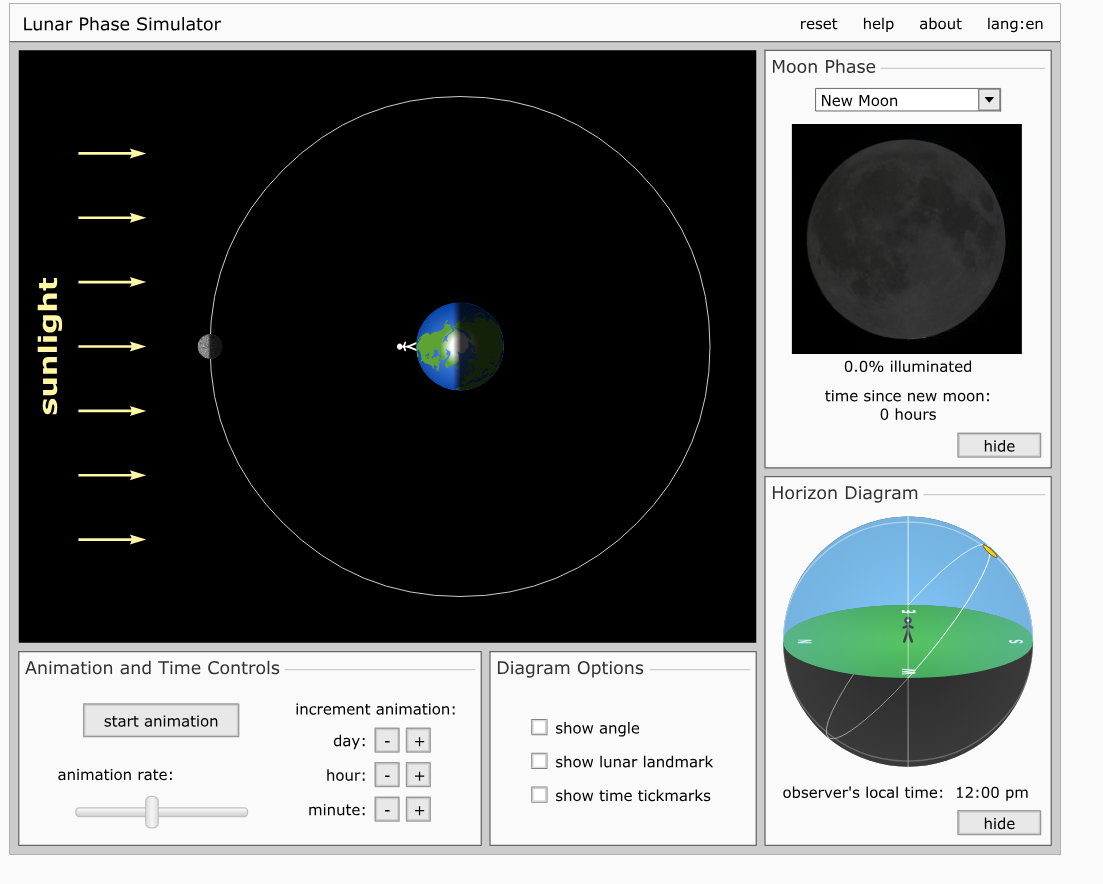
\includegraphics[scale = 0.5]{Imagenes/nebraska.png}
    \centering
    \caption{Simulador de fases de la luna}{Fuente: \cite{UNL2025}}
\end{figure}

Tras una revisión y uso del simulador mencionado, podemos establecer que 
cumple con: 

\textbf{Objetivos:}
\begin{itemize}
    \item Permitir a los estudiantes \textbf{comprender visualmente} cómo la Luna cambia de fase al orbitar la Tierra.
    \item Mostrar la \textbf{relación entre la posición de la luna, la Tierra y la luz solar}.
\end{itemize}

\textbf{Metodología/Tecnología Empleada:}
\begin{itemize}
    \item \textbf{Frontend:} HTML, JavaScript y CSS.
    \item \textbf{Interactividad:} Controles para ajustar el tiempo y ver cómo la Luna cambia de fase en tiempo real.
    \item \textbf{Representación Visual:}
    \begin{itemize}
        \item Simulación orbital en 2D.
        \item Vista del horizonte del observador.
        \item Indicador de fase lunar con porcentaje de iluminación.
    \end{itemize}
\end{itemize}

\textbf{ Resultados o Impactos Obtenidos:}
\begin{itemize}
    \item \textbf{Intuitivo y visualmente atractivo} para la enseñanza en todos los niveles.
    \item No requiere conocimientos previos, ya que se basa en manipulación gráfica.
    \item \textbf{Ideal para principiantes} en astronomía.
\end{itemize}

\addcontentsline{toc}{subsection}{Análisis comparativo}
\subsection*{Análisis comparativo}

A continuación, se realiza una comparativa del simulador de la figgura 4.1 con nuestra propuesta del prototipo:

\begin{table}[H]
    \centering
    \begin{tabular}{|p{4.5cm}|p{5.5cm}|p{5.5cm}|}
        \hline
        \textbf{Criterio} & \textbf{Lunar Phase Simulator (Nebraska)} & \textbf{Propuesta} \\
        \hline
        \textbf{Objetivo} & Visualizar fases lunares de forma interactiva. & Simulación científica con datos reales, material descargable y evaluación del aprendizaje. \\
        \hline
        \textbf{Interactividad} & El usuario ajusta la posición de la Luna manualmente. & El usuario ingresa fechas, obtiene gráficos y responde un \textbf{quiz interactivo} para reforzar el aprendizaje. \\
        \hline
        \textbf{Datos Adicionales} & No proporciona información numérica. & Muestra distancia Tierra-Luna, iluminación y visibilidad, además de permitir la autoevaluación. \\
        \hline
        \textbf{Exportación de Datos} & No permite guardar información. & Genera reportes en PDF para estudiantes con sus resultados del quiz y gráficos de fases lunares. \\
        \hline
        \textbf{Aplicabilidad Educativa} & Bueno para principiantes en astronomía. & Útil tanto para estudiantes como para investigadores, incorporando \textbf{evaluación y retroalimentación} del aprendizaje. \\
        \hline
    \end{tabular}
    \label{tab:comparacion}
    \caption{Comparación entre el Lunar Phase Simulator (Nebraska) y la propuesta del prototipo, incluyendo evaluación interactiva.}
\end{table}


En base a esta comparación, podemos

